\documentclass[a4paper, oneside]{article}

\usepackage[T1]{fontenc}
\usepackage[utf8]{inputenc}
\usepackage[italian]{babel}
\usepackage{graphicx}
\usepackage{soul}
\usepackage{pdflscape}
\usepackage{geometry}

\graphicspath{ {./images/} }
\geometry{
    a4paper,
    left=20mm,
    top=30mm,
    bottom=30mm,
}

\pagenumbering{gobble}
\title{Diario del progetto - Ingegneria del Software}
\date{A.A. 2022/22}
\author{Alessia Crimaldi, Alessio Arcara, Matteo Sacco, Davide Fermi}

%Definizione Variabili
\newcommand\uno{Scrum Master (Alessia Crimaldi), Dev 1 (Alessio Arcara), Dev 2 (Matteo Sacco).}
\newcommand\unoP{Product Owner (Davide Fermi), }
\newcommand\due{Scrum Master (Davide Fermi), Dev 1 (Alessia Crimaldi), Dev 2 (Alessio Arcara).}
\newcommand\dueP{Product Owner (Matteo Sacco), }
\newcommand\tre{Scrum Master (Matteo Sacco), Dev 1 (Davide Fermi), Dev 2 (Alessia Crimaldi).}
\newcommand\treP{Product Owner (Alessio Arcara), }
\newcommand\quattro{Scrum Master (Alessio Arcara), Dev 1 (Matteo Sacco), Dev 2 (Davide Fermi).}
\newcommand\quattroP{Product Owner (Alessia Crimaldi), }
\newcommand\cinque{Scrum Master (Alessia Crimaldi), Dev 1 (Alessio Arcara), Dev 2 (Matteo Sacco).}
\newcommand\cinqueP{Product Owner (Davide Fermi), }

\begin{document}
    \begin{landscape}
        \begin{titlepage}
            \maketitle
        \end{titlepage}
        \newpage
        %%%%%%%%%%%%%%%%%%
        %                %
        %    SPRINT 1    %
        %                %
        %%%%%%%%%%%%%%%%%%
        \section{SPRINT 01}
        \begin{itemize}
            \item Inizio sprint: \textit{08/01/2023}
            \item Fine sprint: \textit{14/01/2023}
        \end{itemize}
        \begin{itemize}
            \item \textbf{Sprint Goal (SG):} \\
            \begin{indent}
                \newline Permettere ad un visitatore di utilizzare tutte le funzionalita' base dell'app, ossia di avere una corretta ed efficace importazione e gestione del catalogo carte con le relative ricerche e visualizzazione dei dettagli della carta.\\
            \end{indent}
        \end{itemize}
        \begin{itemize}
            \item \textbf{Ruoli:}\\
            \textbf{Product Owner:} Davide Fermi\\
            \textbf{Scrum Master:} Alessia Crimaldi\\
            \textbf{Development team:} Alessio Arcara, Matteo Sacco\\
        \end{itemize}
        \vspace{2mm} %5mm vertical space
        \subsection{Sprint Planning (S01)}
        \textbf{Data:} 08/01/2023\\
        \textbf{Durata:} 95 min.\\
        \textbf{Partecipanti:} \unoP \uno\\
        \newline La riunione inizia con la presentazione da parte del Product Owner del Product Backlog, introducendo le User Stories e con le relative priorità. Viene proposto dallo Scrum Master di utilizzare il metodo ' Planning Poker' per stablire gli Story Points per ogni User Stories e viene selezionato uno strumento online per facilitare l'utilizzo del metodo. Viene concordato dal team, tra le scale disponibili, di utilizzare la sequenza di Fibonacci modificata (0  1/2  1  2  3  5  8  13  20  40  100  ?  -tazzina di caffè-). Successivamente si è passato a stimare l'effort per ogni User Stories per poi definire l'effort totale settiminale per lo sviluppo. E' stato successivamente popolato lo Sprint Backlog a cura degli sviluppatori e dello Scrum Master, fino al raggiungimento dell'effort totale precedentemente stimato. Ogni singola User Stories presente nello Sprint Backlog è stata successivamente raffinata in tasks di sviluppo, per ognuno dei quali è stato stimato un effort per l'implementazione.

        \newpage
        \subsection{Stato board dopo lo Sprint Planning (S01):}
        \small
        \def\arraystretch{2}%
        \begin{tabular}{ | p{6.5cm} | p{3.5cm} | p{8cm} | p{2.4cm} | p{2.4cm}| }
            \hline
            \textbf{UC raffinati}
            & \textbf{Product Backlog}
            & \textbf{Sprint Backlog}
            & \textbf{Sprint In progress}
            & \textbf{Sprint Done} \\
            \hline
            \textbf{UC01:} Come visitatore voglio selezionare un gioco e vedere l'elenco di tutte le sue carte
            &  & \textbf{Task1 [UC01]\#2:} Creare il modello per le carte di tutti i giochi & & \\
            \hline
            \textbf{UC02:} Come visitatore voglio poter fare delle ricerche per vedere un elenco di carte filtrato
            &  & \textbf{Task2 [UC01]\#3:} Importare dai JSON le carte dei giochi & & \\
            \hline
            \textbf{UC03:} Come visitatore voglio selezionare una carta e vederne i dettagli
            & & \textbf{Task3 [UC01]\#4:} Inizializzare il DB con i JSON caricati & & \\
            \hline
            & & \textbf{Task4 [UC01]\#5:} Creare RemoteService per fetch delle carte di quel gioco & & \\
            \hline
            & & \textbf{Task5 [UC01]\#6:} Creare HomeView per la visualizzazione delle carte & & \\
            \hline
            & & \textbf{Task6 [UC01]\#7:} Creare Composite Card per la visualizzazione carta & & \\
            \hline
            & & \textbf{Task1 [UC02]\#10:} Creare filtri specifici di quel gioco & & \\
            \hline
            & & \textbf{Task2 [UC02]\#11:} Filtrare l'array delle carte in base ai filtri specificati & & \\
            \hline
            & & \textbf{Task3 [UC02]\#12:} Rimuovere dalla pagina HomeView le carte che non corrispondono ai filtri & & \\
            \hline
            & & \textbf{Task1 [UC03]\#14:} Creazione CardPlace & & \\
            \hline
            & & \textbf{Task2 [UC03]\#15:} Connessione RemoteService FetchCard nel caso l'assunzione sia errata & & \\
            \hline
            & & \textbf{Task3 [UC03]\#16:} Creazione CardView e popolamento delle informazioni & & \\
            \hline
            & & \textbf{Task4 [UC03]\#17:} Gestione del cambio di pagina da HomeView a CardView & & \\
            \hline
        \end{tabular}

        \newpage
        \normalsize
        \subsection{Daily Scrum (S01):}
        \begin{itemize}
            \item \textbf{Data:} 09/01/2023
            \newline \textbf{Durata:} 15 min.
            \newline \textbf{Partecipanti:} Scrum Master (Alessia Crimaldi), Dev 1 (Alessio Arcara).
            \newline \textbf{Percezione attuale dello SG:} Positiva (Dev 1)
        \end{itemize}
        \begin{itemize}
            \item \textbf{Data:} 10/01/2023
            \newline \textbf{Durata:} 15 min.
            \newline \textbf{Partecipanti:} \uno
            \newline \textbf{Percezione attuale dello SG:} Negativa (Dev 1), Positiva (Dev 2)
        \end{itemize}
        \begin{itemize}
            \item \textbf{Data:} 11/01/2023
            \newline \textbf{Durata:} 15 min.
            \newline \textbf{Partecipanti:} \uno
            \newline \textbf{Percezione attuale dello SG:} Negativa (Dev 1), Negativa (Dev 2)
        \end{itemize}
        \begin{itemize}
            \item \textbf{Data:} 12/01/2023
            \newline \textbf{Durata:} 15 min.
            \newline \textbf{Partecipanti:} \uno
            \newline \textbf{Percezione attuale dello SG:} Negativa (Dev 1), Negativa (Dev 2)
        \end{itemize}
        \begin{itemize}
            \item \textbf{Data:} 13/01/2023
            \newline \textbf{Durata:} 12 min.
            \newline \textbf{Partecipanti:} \uno
            \newline \textbf{Percezione attuale dello SG:} Negativa (Dev 1), Negativa (Dev 2)
        \end{itemize}
        \begin{itemize}
            \item \textbf{Data:} 14/01/2023
            \newline \textbf{Durata:} 10 min.
            \newline \textbf{Partecipanti:} \uno
            \newline \textbf{Percezione attuale dello SG:} Negativa (Dev 1), Negativa (Dev 2)
        \end{itemize}
        \vspace{2mm} %5mm vertical space
        \textbf{Note:} Si è cercato di mantenere i daily entro i 10 minuti, nei quali il team di sviluppo, condotti dallo Scrum Master, espongono quanto fatto, quanto hanno in progetto di fare e i principali problemi riscontrati. Al termine, lo Scrum master chiede una percezione dello Sprint Goal e mostra il BurnDown Chart aggiornato.

        \newpage
        \subsection{Stato Board finale (S01):}
        \small
        \def\arraystretch{2}%
        \begin{tabular}{ | p{5cm} | p{3cm} | p{5cm} | p{5cm} | p{5cm}| }
            \hline
            \textbf{UC raffinati}
            & \textbf{Product Backlog}
            & \textbf{Sprint Backlog}
            & \textbf{Sprint In progress}
            & \textbf{Sprint Done} \\
            \hline
            \textbf{UC01:} Come visitatore voglio selezionare un gioco e vedere l'elenco di tutte le sue carte
            & \textbf{UC04:}  Come utente voglio potermi autenticare per gestire i miei mazzi di carte & \textbf{Task1 [UC03]\#14:} Creazione CardPlace
            & \textbf{Task2 [UC02]\#11:} Filtrare l'array delle carte in base ai filtri specificati
            & \textbf{Task1 [UC01]\#2:} Creare il modello per le carte di tutti i giochi \\
            \hline
            \textbf{UC02:} Come visitatore voglio poter fare delle ricerche per vedere un elenco di carte filtrato
            & \textbf{UC05:}  Come utente voglio poter aggiungere le mie carte reali al mazzo delle possedute & \textbf{Task2 [UC03]\#15:} Connessione RemoteService FetchCard nel caso l'assunzione sia errata
            & \textbf{Task3 [UC02]\#12:} Rimuovere dalla pagina HomeView le carte che non corrispondono ai filtri
            & \textbf{Task4 [UC01]\#5:} Creare RemoteService per fetch delle carte di quel gioco \\
            \hline
            \textbf{UC03:} Come visitatore voglio selezionare una carta e vederne i dettagli
            & \textbf{UC06:} Come utente voglio poter visualizzare il contenuto del mazzo delle possedute & \textbf{Task3 [UC03]\#16:} Creazione CardView e popolamento delle informazioni
            & \textbf{Task6 [UC01]\#7:} Creare Composite Card per la visualizzazione carta
            & \textbf{Task5 [UC01]\#6:} Creare HomeView per la visualizzazione delle carte \\
            \hline
            & \textbf{UC07:} Come utente voglio poter aggiungere le carte reali che desidero al mazzo delle desiderate  & \textbf{Task4 [UC03]\#17:} Gestione del cambio di pagina da HomeView a CardView
            & & \textbf{Task2 [UC01]\#3:} Importare dai JSON le carte dei giochi \\
            \hline
            & & & & \textbf{Task1 [UC02]\#10:} Creare filtri specifici di quel gioco  \\
            \hline
            & & & & \textbf{Task3 [UC01]\#4:} Inizializzare il DB con i JSON caricati \\
            \hline
        \end{tabular}

        \newpage
        \normalsize
        \subsection{Sprint Review (S01):}
        \begin{itemize}
            \item \textbf{Data:} 15/01/2023
            \newline \textbf{Durata:} 105 min.
            \newline \textbf{Partecipanti:} \unoP \uno
            \newline
            \newline I developers mostrano al Product Owner una Demo di quanto finora prodotto. Si evidenzia come non sia stato possibile sviluppare tutte le funzionalità richieste dallo Sprint Goal. Si analizzano quindi le principali cause che hanno portato a questo problema, evidenziando come il framework GWT abbia introdotto della complessità nell'implementazione. Il Product Owner decide quindi che non ci sono le condizioni sufficienti per procedere ad un rilascio, comprendendo comunque le difficoltà riscontrate, ma chiedendo uno sforzo maggiore per lo sprint successivo, al fine di poter presentare un prodotto rilasciabile. Non vengono evidenziati particolari problematiche di collaborazione e comunicazione all'interno del team.

            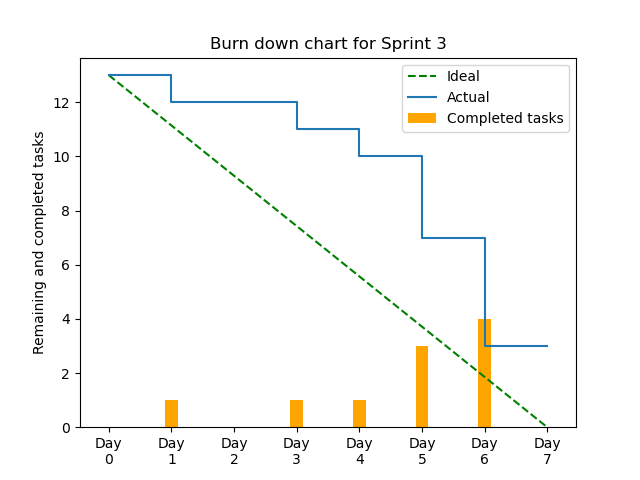
\includegraphics[scale=0.8]{Sprint03_BurnDownChart}
            --- METTERE QUELLO CORRETTO!!! ---

        \end{itemize}

        \newpage
        \subsection{Sprint Retrospective (S01):}
        \begin{itemize}
            \item \textbf{Data:} 15/01/2023
            \newline \textbf{Durata:} 70 min.
            \newline \textbf{Partecipanti:} \unoP \uno
            \newline
            \newline Lo Scrum Master chiede a tutti i membri di evidenziare gli aspetti positivi dello sprint appena concluso. Si sottolinea come il Planning Poker abbia permesso al team di lavorare insieme e dinamicamente, confrontandosi e discutendo, per giungere a una decisione condivisa, nonostante il fatto che le opinioni individuali iniziali fossero a volte distanti. Si riconosce come il lavoro di formazione durante la fase di inception abbia reso più veloce lo sviluppo, ma non abbastanza. Per quanto riguarda gli aspetti negativi, emerge, oltre a quanto già discusso nello Sprint Review, che nonostante la percezione sia quasi da subito parsa negativa, non è stata applicata nessuna azione correttiva. Si decide quindi per il futuro, qualora si ripresentasse una situazione simile, di richiedere un confronto con il Product Owner e valutare se sia necessario rivedere lo Sprint Backlog, nel tentativo di migliorare dinamicamente il flusso di lavoro.
        \end{itemize}

        \newpage
        %%%%%%%%%%%%%%%%%%
        %                %
        %    SPRINT 2    %
        %                %
        %%%%%%%%%%%%%%%%%%
        \section{SPRINT 02}
        \begin{itemize}
            \item Inizio sprint: \textit{15/01/2023}
            \item Fine sprint: \textit{22/01/2023}
        \end{itemize}
        \begin{itemize}
            \item \textbf{Sprint Goal (SG):}\\
            \begin{indent}
                \newline Permettere ad un visitatore di autenticarsi come utente e permettere ad un visitatore di effettuare una ricerca di carte dal catalogo potendo applicanre dei filtri.\\
            \end{indent}
        \end{itemize}
        \begin{itemize}
            \item \textbf{Ruoli:}\\
            \textbf{Product Owner:} Matteo Sacco \\
            \textbf{Scrum Master:} Davide Fermi \\
            \textbf{Development team:} Alessio Arcara, Alessia Crimaldi \\
        \end{itemize}
        \vspace{2mm} %5mm vertical space
        \subsection{Sprint Planning (S02)}
        \textbf{Data:} 15/01/2023 \\
        \textbf{Durata:} 85 min. \\
        \textbf{Partecipanti:} \dueP \due \\
        \newline Il Product Owner prensenta il Product Backlog aggiornato, descrivendo dettagliatamente gli UC presenti. Lo Scrum Master introduce il Planning Poker e vengono quindi assegnati gli Story Points dinamicamente e in maniera condivisa.  Il team stima l'effort per ogni User Story e successivamente l'effort totale settimanale disponibile. Esse vengono quindi inserite nello Sprint Backlog, fino al raggiungimento dell'effort disponibile.  Gli sviluppatori effettuano la suddivisione delle singole User Stories in task più dettagliati, per una maggiore comprensione e pianificazione. Lo Scrum master concorda con il team la pianificazione dei daily e li inserisce a calendario.

        \newpage
        \subsection{Stato board dopo lo Sprint Planning (S02):}
        \small
        \def\arraystretch{2}%
        \begin{tabular}{ | p{6cm} | p{3.2cm} | p{7.8cm} | p{3.6cm} | p{2.2cm}| }
            \hline
            \textbf{UC raffinati}
            & \textbf{Product Backlog}
            & \textbf{Sprint Backlog}
            & \textbf{Sprint In progress}
            & \textbf{Sprint Done} \\
            \hline
            \hline
            \textbf{UC01:} Come visitatore voglio selezionare un gioco e vedere l'elenco di tutte le sue carte & \textbf{UC06:} Come utente voglio poter visualizzare il contenuto del mazzo delle possedute & \textbf{Task1 [UC03]\#14:} Creazione CardPlace & \textbf{Task2 [UC02]\#11:} Filtrare l'array delle carte in base ai filtri specificati   & \\
            \hline
            \textbf{UC02:} Come visitatore voglio poter fare delle ricerche per vedere un elenco di carte filtrato &  \textbf{UC07:} Come utente voglio poter aggiungere le carte reali che desidero al mazzo delle desiderate  & \textbf{Task2 [UC03]\#15:} Connessione RemoteService FetchCard nel caso l'assunzione sia errata &  \textbf{Task3 [UC02]\#12:} Rimuovere dalla pagina HomeView le carte che non corrispondono ai filtri & \\
            \hline
            \textbf{UC03:}  Come visitatore voglio selezionare una carta e vederne i dettagli &  & \textbf{Task3 [UC03]\#16:} Creazione CardView e popolamento delle informazioni  & \textbf{Task6 [UC01]\#7:}  Creare Composite Card per la visualizzazione carta &\\
            \hline
            \textbf{UC04:}  Come utente voglio potermi autenticare per gestire i miei mazzi di carte & & \textbf{Task4 [UC03]\#17:} Gestione del cambio di pagina da HomeView a CardView & & \\
            \hline
            \textbf{UC05:}  Come utente voglio poter aggiungere le mie carte reali al mazzo delle possedute & & \textbf{Task1 [UC04]\#32:} Creare Authentication view per Login/registrazione  & & \\
            \hline
            & & \textbf{Task2 [UC04]\#33:} Creare RPC SignUp & & \\
            \hline
            & & \textbf{Task3 [UC04]\#34:} Creare RPC SignIn  & & \\
            \hline
            & & \textbf{Task4 [UC04]\#35:} Gestire la sessione  & & \\
            \hline
            & & \textbf{Task1 [UC05]\#36:} Creare modello per strutturare i mazzi predefiniti (possedute/desiderate) e il loro contenuto  & & \\
            \hline
            & & \textbf{Task2 [UC05]\#54:} \st{Creare mappa dei mazzi su MapDB (ex \#37)} (*) & & \\

            \hline
            & & --- continua --- & & \\
            \hline
        \end{tabular}

        \newpage
        \noindent
        \begin{tabular}{ | p{6cm} | p{3.2cm} | p{7.8cm} | p{3.6cm} | p{2.2cm}| }
            \hline
            \textbf{UC raffinati}
            & \textbf{Product Backlog}
            & \textbf{Sprint Backlog}
            & \textbf{Sprint In progress}
            & \textbf{Sprint Done} \\
            \hline
            \hline
            & & \textbf{Task3 [UC05]\#63:} \st{Creare metodo statico in AuthService per controllare validit\'{a} token e restituire email utente (ex \#38)}  (*)   & & \\
            \hline
            & & \textbf{Task4 [UC05]\#55:} \st{Modificare RPC signup per aggiungere il mazzo delle possedute alla creazione dell'utente (ex \#39)}  (*)  & & \\
            \hline
            & & \textbf{Task5 [UC05]\#56:} \st{Creare RPC per inserire una carta fisica nel mazzo delle possedute dell'utente (ex \#40)}  (*)   & & \\
            \hline
            & & \textbf{Task6 [UC05]\#57:} \st{Modificare CardView per poter aggiungere la carta al mazzo delle possedute (ex \#41)}  (*)   & & \\
            \hline
        \end{tabular}
        \\
        \begin{flushright}
        (*) Vedi nota pagina successiva.
        \end{flushright}

        \newpage
        \normalsize
        \subsection{Daily Scrum (S02):}
        \begin{itemize}
            \item \textbf{Data:} 16/01/2023
            \newline \textbf{Durata:} 20 min.
            \newline \textbf{Partecipanti:} \due
            \newline \textbf{Percezione attuale dello SG:} Positiva (Dev 1), Positiva (Dev 2)
        \end{itemize}
        \begin{itemize}
            \item \textbf{Data:} 17/01/2023
            \newline \textbf{Durata:} 15 min.
            \newline \textbf{Partecipanti:} \due
            \newline \textbf{Percezione attuale dello SG:} Positiva (Dev 1), Positiva (Dev 2)
        \end{itemize}
        \begin{itemize}
            \item \textbf{Data:} 18/01/2023
            \newline \textbf{Durata:} 15 min.
            \newline \textbf{Partecipanti:} \due
            \newline \textbf{Percezione attuale dello SG:} Positiva (Dev 1), Positiva (Dev 2)
        \end{itemize}
        \begin{itemize}
            \item \textbf{Data:} 19/01/2023
            \newline \textbf{Durata:} 15 min.
            \newline \textbf{Partecipanti:} \due
            \newline \textbf{Percezione attuale dello SG:} Negativa (Dev 1), Negativiva (Dev 2)
            \newline \textbf{Note:} Viene richiesta convocazione PO per rivalutazione Sprint Backlog
        \end{itemize}
        \begin{itemize}
            \item \textbf{Data:} 20/01/2023
            \newline \textbf{Durata:} 45 min.
            \newline \textbf{Partecipanti:} \dueP \due
            \newline \textbf{Percezione attuale dello SG:} Positiva (Dev 1), Positiva (Dev 2)
            \newline \textbf{Note:} Viene ridiscusso sprint backlog con PO in base a problematiche emerse(*).
        \end{itemize}
        \begin{itemize}
            \item \textbf{Data:} 21/01/2023
            \newline \textbf{Durata:} 15 min.
            \newline \textbf{Partecipanti:} \due
            \newline \textbf{Percezione attuale dello SG:} Negativa (Dev 1), Positiva (Dev 2)
        \end{itemize}
        \textbf{Note:} Si è cercato di mantenere i daily entro i 10 minuti, nei quali il team di sviluppo, condotti dallo Scrum Master, espongono quanto fatto, quanto hanno in progetto di fare e i principali problemi riscontrati. Al termine, lo Scrum master chiede una percezione dello Sprint Goal e mostra il BurnDown Chart aggiornato. \\
        (*) Valutando che non era possibile portare a termine tutti i task assegnati nello Spint Backlog per sopraggiunti problematiche bloccanti per limiti implementativi, durante lo sprint è stato rimodulato il carico di lavoro.

        \newpage
        \newpage
        \subsection{Stato Board finale (S02):}
        \small
        \def\arraystretch{2}%
        \begin{tabular}{ | p{4.5cm} | p{4cm} | p{4cm} | p{5cm} | p{5.5cm}| }
            \hline
            \textbf{UC raffinati}
            & \textbf{Product Backlog}
            & \textbf{Sprint Backlog}
            & \textbf{Sprint In progress}
            & \textbf{Sprint Done} \\
            \hline
            \hline
            \textbf{UC01:} Come visitatore voglio selezionare un gioco e vedere l'elenco di tutte le sue carte & \textbf{[UC06]:} Come utente voglio poter visualizzare il contenuto del mazzo delle possedute & & \textbf{Task3 [UC03]\#16:} Creazione CardView e popolamento delle informazioni  & \textbf{Task6 [UC01]\#7:}  Creare Composite Card per la visualizzazione carta \\
            \hline
            \textbf{UC02:} Come visitatore voglio poter fare delle ricerche per vedere un elenco di carte filtrato & \textbf{UC07:} Come utente voglio poter aggiungere le carte reali che desidero al mazzo delle desiderate &  &   & \textbf{Task2 [UC02]\#11:} Filtrare l'array delle carte in base ai filtri specificati \\
            \hline
            \textbf{UC03:} Come visitatore voglio selezionare una carta e vederne i dettagli & \textbf{UC08:} Come utente voglio poter rimuovere le carte reali che non desidero più dal mazzo delle desiderate & & & \textbf{Task3 [UC02]\#12:} Rimuovere dalla pagina HomeView le carte che non corrispondono ai filtri \\
            \hline
            \textbf{UC04:}  Come utente voglio potermi autenticare per gestire i miei mazzi di carte & \textbf{UC09:} Come utente voglio poter proporre una richiesta di scambio per una o più carte reali possedute da un altro utente &  & & \textbf{Task2 [UC03]\#15:} Connessione RemoteService FetchCard nel caso l'assunzione sia errata \\
            \hline
            \textbf{UC05:}  Come utente voglio poter aggiungere le mie carte reali al mazzo delle possedute & \textbf{UC10:} Come utente voglio poter accettare una richiesta di scambio di un altro utente & & & \textbf{Task4 [UC03]\#17:} Gestione del cambio di pagina da HomeView a CardView \\
            \hline
            & &  & & \textbf{Task1 [UC03]\#14:} Creazione CardPlace \\
            \hline
            & &  & & \textbf{Task1 [UC04]\#32:} Creare Authentication view per Login/registrazione \\
            \hline
            & &   & & \textbf{Task2 [UC04]\#33:} Creare RPC SignUp \\
            \hline
            & &   & & \textbf{Task3 [UC04]\#34:} Creare RPC SignIn  \\
            \hline
            & & --- continua --- & & \\
            \hline
        \end{tabular}

        \newpage
        \noindent
        \begin{tabular}{ | p{5cm} | p{3cm} | p{5cm} | p{5cm} | p{5cm}| }
            \hline
            \textbf{UC raffinati}
            & \textbf{Product Backlog}
            & \textbf{Sprint Backlog}
            & \textbf{Sprint In progress}
            & \textbf{Sprint Done} \\
            \hline
            \hline
            & &   & & \textbf{Task4 [UC04]\#35:} Gestire la sessione\\
            \hline
            & &   & & \textbf{Task1 [UC05]\#36:} Creare modello per strutturare i mazzi predefiniti (possedute/desiderate) e il loro contenuto\\
            \hline
        \end{tabular}

        \newpage
        \normalsize
        \subsection{Sprint Review (S02):}
        \begin{itemize}
            \item \textbf{Data:} 22/01/2023
            \newline \textbf{Durata:} 105 min.
            \newline \textbf{Partecipanti:}  \dueP \due
            \newline
            \newline Viene prima effettuata la Demo da parte dei devolopers. Nella discussione sull'andamento dello Sprint, emerge come sia necessario migliorare la definizione dei tasks, aumentandone il dettaglio e quindi suddividendo i task grandi in molti sub-tasks più piccoli. Questo anche per evitare Pull Request troppo grosse (e quindi più complicate da gestire, con un pericoloso effetto cascata sul Team). Si evidenzia che il Product Backlog andrebbe continuamente popolato e raffinato durante tutto lo sprint. Ci sono critiche e chiarimenti rigurardo effort di alcuni elementi del team. Viene chiesta in generale anche più precisione nella definizione dello Sprint Backlog, in quanto anche questa settimana si stava rischiando di non rilasciare.Da alcuni membri viene sottolineato come il livello di dettaglio dell'attuale manuale dello sviluppatore sia troppo profondo, richiedendo sforzi per taluni eccessivi rispetto a quanto preventivato. Il Product Owner al termine della riunione, decide che lo sprint si è concluso positivamente ed è possibile rilasciare, incaricando i developers delle pratiche formali di rilascio e della definizione delle Releas Notes.

            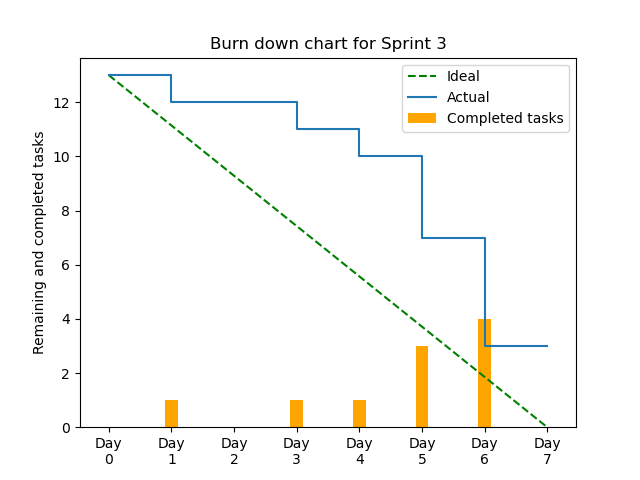
\includegraphics[scale=0.8]{Sprint03_BurnDownChart}
            --- METTERE QUELLO CORRETTO!!! ---
        \end{itemize}

        \newpage
        \subsection{Sprint Retrospective (S02):}
        \begin{itemize}
            \item \textbf{Data:} 22/01/2023
            \newline \textbf{Durata:} 70 min.
            \newline \textbf{Partecipanti:}  \dueP \due
            \newline
            \newline Lo Scrum Master chiede a tutti i membri di evidenziare gli aspetti positivi dello sprint appena concluso. Si sottolinea come una più profonda conoscenza del framework abbia agevolato e velocizzato gli sviluppi e viene confermata l'importanza e i vantaggi dell'approccio Test Driven Design, nonostante l'ingente quantità di effort che richiede nell'implementazione iniziale. Viene poi proposto un nuovo ordine e dettaglio della Definition of Done (tutti si concorda a riguardo e viene subito implementato nelle actions di GitHub). Viene proposto di utilizzare la tecnica del "Pair Programming" per agevolare e accellerare l'autonomia dei nuovi sviluppatori e per diffondere più velocemente conoscenza. Infine si concorda di utilizzare il metodo "velocity" per la definizione dello Sprint Backlog, al fine di cercare di organizzare più efficacemente la pianificazione dello Sprint successivo.
        \end{itemize}

        \newpage
        %%%%%%%%%%%%%%%%%%
        %                %
        %    SPRINT 3    %
        %                %
        %%%%%%%%%%%%%%%%%%
        \section{SPRINT 03}
        \begin{itemize}
            \item Inizio sprint: \textit{22/01/2023}
            \item Fine sprint: \textit{29/01/2023}
        \end{itemize}
        \begin{itemize}
            \item \textbf{Sprint Goal (SG):} \\
            \begin{indent}
                \newline Il sistema deve permettere all’utente di aggiungere carte da gioco che possiede nella realtà al proprio account e deve permettere all’utente di visualizzare carte da gioco che possiede nella realtà aggiunte al proprio account. \\
            \end{indent}
        \end{itemize}
        \begin{itemize}
            \item \textbf{Ruoli:}\\
            \textbf{Product Owner:} Alessio Arcara \\
            \textbf{Scrum Master:} Matteo Sacco \\
            \textbf{Development team:} Davide Fermi, Alessia Crimaldi \\
        \end{itemize}
        \vspace{2mm} %5mm vertical space
        \subsection{Sprint Planning (S03)}
        \textbf{Data:} 22/01/2023\\
        \textbf{Durata:} 75 min.\\
        \textbf{Partecipanti:} \treP \tre \\
        \newline La riunione inizia con la spiegazione del Product Backlog aggiornato da parte del Product Owner, con definizione delle priorità delle singole User Stories. Viene come di consueto applicata la strategia del Planning Poker tra i membri del team, utilizzando come scala la stessa già impiegata nei planning precedenti e con il consueto flusso di pianificazione (stima l'effort per ogni user stories, definizione effort totale settiminale, popolamento dello Sprint Backlog, raffinamento User Stories e produzione tasks di sviluppo, con stima effort). Come deciso precedentemente, l'approccio di pianificazione per questo nuovo sprint si baserà sulla 'velocity'.
        \newline Come proposto nello Sprint Retrospective, per la durata dello Sprint e in particolar modo nelle fasi iniziali, verrà adottata una strategia di Pair Programming di tipo "Navigator-Driver", al fine di facilitare il passaggio di conoscenza.

        \newpage
        \subsection{Stato board dopo lo Sprint Planning (S03):}
        \small
        \def\arraystretch{2}%
        \begin{tabular}{ | p{6cm} | p{5cm} | p{6.2cm} | p{3.8cm} | p{2cm}| }
            \hline
            \textbf{UC raffinati}
            & \textbf{Product Backlog}
            & \textbf{Sprint Backlog}
            & \textbf{Sprint In progress}
            & \textbf{Sprint Done} \\
            \hline
            \hline
            \textbf{UC01:} Come visitatore voglio selezionare un gioco e vedere l'elenco di tutte le sue carte & \textbf{UC07:} Come utente voglio poter aggiungere le carte reali che desidero al mazzo delle desiderate &\textbf{Task4 [UC06]\#61:} Creare pagina per visualizzare il mazzo delle possedute (Place, Activity e View) & \textbf{Task1 [UC03]\#16:} Creazione CardView e popolamento delle informazioni &
            \\
            \hline
            \textbf{UC02:} Come visitatore voglio poter fare delle ricerche per vedere un elenco di carte filtrato & \textbf{UC08:} Come utente voglio poter rimuovere le carte reali che non desidero più dal mazzo delle desiderate & \textbf{Task2 [UC05]\#54:} Creare mappa dei mazzi su MapDB & & \\
            \hline
            \textbf{UC03:} Come visitatore voglio selezionare una carta e vederne i dettagli & \textbf{UC09:} Come utente voglio poter proporre una richiesta di scambio per una o più carte reali possedute da un altro utente & \textbf{Task3 [UC05]\#55:} Modificare RPC signup per aggiungere il mazzo delle possedute alla creazione dell'utente & & \\
            \hline
            \textbf{UC04:}  Come utente voglio potermi autenticare per gestire i miei mazzi di carte & \textbf{UC10:} Come utente voglio poter accettare una richiesta di scambio di un altro utente & \textbf{Task4 [UC05]\#56:} Creare RPC per inserire una carta fisica nel mazzo delle possedute dell'utente & & \\
            \hline
            \textbf{UC05:} Come utente voglio poter aggiungere le mie carte reali al mazzo delle possedute & & \textbf{Task5 [UC05]\#57:} Modificare CardView per poter aggiungere la carta al mazzo delle possedute & & \\
            \hline
            \textbf{UC06:} Come utente voglio poter visualizzare il contenuto del mazzo delle possedute & & \textbf{Task6 [UC05]\#63:} Creare metodo statico in AuthService per controllare validità token e restituire email utente & & \\
            \hline
            & & \textbf{Task7 [UC05]\#71:} Modificare modello PhysicalCard in modo che status sia un valore numerico da 1 a 5 e non una stringa & & \\
            \hline

            & & \textbf{Task1 [UC06]\#58:} Creare modello carta fisica che al posto di cardId restituirà sia il titolo della carta che cardId & & \\
            \hline
            & & \textbf{Task2 [UC06]\#59:} Creare RPC per poter visualizzare la lista di carte reali contenute nel mazzo delle possedute & & \\
            \hline
            & & \textbf{Task3 [UC06]\#60:} Inserire hyperlink nel menù laterale (visibile solo se autenticato) & & \\
            \hline
        \end{tabular}

        \newpage
        \normalsize
        \subsection{Daily Scrum (S03):}
        \begin{itemize}
            \item \textbf{Data:} 23/01/2023
            \newline \textbf{Durata:} 15 min.
            \newline \textbf{Partecipanti:} \tre
            \newline \textbf{Percezione attuale dello SG:} Positiva (Dev 1), Positiva (Dev 2)
        \end{itemize}
        \begin{itemize}
            \item \textbf{Data:} 24/01/2023
            \newline \textbf{Durata:} 15 min.
            \newline \textbf{Partecipanti:} \tre
            \newline \textbf{Percezione attuale dello SG:} Positiva (Dev 1), Positiva (Dev 2)
        \end{itemize}
        \begin{itemize}
            \item \textbf{Data:} 25/01/2023
            \newline \textbf{Durata:} 15 min.
            \newline \textbf{Partecipanti:} \tre
            \newline \textbf{Percezione attuale dello SG:} Positiva (Dev 1), Positiva (Dev 2)
        \end{itemize}
        \begin{itemize}
            \item \textbf{Data:} 26/01/2023
            \newline \textbf{Durata:} 20 min.
            \newline \textbf{Partecipanti:} \tre
            \newline \textbf{Percezione attuale dello SG:} Positiva (Dev 1), Positiva (Dev 2)
        \end{itemize}
        \begin{itemize}
            \item \textbf{Data:} 27/01/2023
            \newline \textbf{Durata:} 15 min.
            \newline \textbf{Partecipanti:} \tre
            \newline \textbf{Percezione attuale dello SG:} Negativa (Dev 1), Negativa (Dev 2)
        \end{itemize}
        \begin{itemize}
            \item \textbf{Data:} 28/01/2023
            \newline \textbf{Durata:} 15 min.
            \newline \textbf{Partecipanti:} \tre
            \newline \textbf{Percezione attuale dello SG:} Negativa (Dev 1), Negativa (Dev 2)
        \end{itemize}
        \vspace{2mm} %5mm vertical space
        \textbf{Note:} Si è cercato di mantenere i daily entro i 10 minuti, nei quali il team di sviluppo, condotti dallo Scrum Master, espongono quanto fatto, quanto hanno in progetto di fare e i principali problemi riscontrati. Al termine, lo Scrum master chiede una percezione dello Sprint Goal e mostra il BurnDown Chart aggiornato.

        \newpage
        \subsection{Stato Board finale (S03):}
        \small
        \def\arraystretch{2}%
        \begin{tabular}{ | p{4.5cm} | p{4.3cm} | p{3.7cm} | p{5cm} | p{5.5cm}| }
            \hline
            \textbf{UC raffinati}
            & \textbf{Product Backlog}
            & \textbf{Sprint Backlog}
            & \textbf{Sprint In progress}
            & \textbf{Sprint Done} \\
            \hline
            \hline
            \textbf{UC01:} Come visitatore voglio selezionare un gioco e vedere l'elenco di tutte le sue carte & \textbf{UC07:} Come utente voglio poter aggiungere le carte reali che desidero al mazzo delle desiderate & & \textbf{Task5 [UC05]\#57:} Modificare CardView per poter aggiungere la carta al mazzo delle possedute &
            \textbf{Task1 [UC03]\#16:} Creazione CardView e popolamento delle informazioni \\
            \hline
            \textbf{UC02:} Come visitatore voglio poter fare delle ricerche per vedere un elenco di carte filtrato &  \textbf{UC08:} Come utente voglio poter rimuovere le carte reali che non desidero più dal mazzo delle desiderate & & \textbf{Task2 [UC06]\#59:} Creare RPC per poter visualizzare la lista di carte reali contenute nel mazzo delle possedute  & \textbf{Task2 [UC05]\#54:} Creare mappa dei mazzi su MapDB \\
            \hline
            \textbf{UC03:} Come visitatore voglio selezionare una carta e vederne i dettagli  & \textbf{UC09:} Come utente voglio poter proporre una richiesta di scambio per una o più carte reali possedute da un altro utente & & \textbf{Task4 [UC06]\#61:} Creare pagina per visualizzare il mazzo delle possedute (Place, Activity e View) & \textbf{Task3 [UC05]\#55:} Modificare RPC signup per aggiungere il mazzo delle possedute alla creazione dell'utente \\
            \hline
            \textbf{UC04:}  Come utente voglio potermi autenticare per gestire i miei mazzi di carte & \textbf{UC10:} Come utente voglio poter accettare una richiesta di scambio di un altro utente & & & \textbf{Task4 [UC05]\#56:} Creare RPC per inserire una carta fisica nel mazzo delle possedute dell'utente \\
            \hline
            \textbf{UC05:} Come utente voglio poter aggiungere le mie carte reali al mazzo delle possedute & \textbf{UC11:} Come utente voglio poter rimuovere le mie carte reali dal mazzo delle possedute & & &  \textbf{Task3 [UC06]\#60:} Inserire hyperlink nel menù laterale (visibile solo se autenticato)  \\
            \hline
            \textbf{UC06:} Come utente voglio poter visualizzare il contenuto del mazzo delle possedute & \textbf{UC12:} Come utente voglio poter rifiutare una richiesta di scambio di un altro utente & & & \textbf{Task6 [UC05]\#63:} Creare metodo statico in AuthService per controllare validità token e restituire email utente \\
            \hline
            & \textbf{UC13:} Come utente voglio poter modificare le proprietà di una mia carta reale aggiunta al mazzo delle possedute & & & \textbf{Task7 [UC05]\#71:} Modificare modello PhysicalCard in modo che status sia un valore numerico da 1 a 5 e non una stringa \\
            \hline
            &  & ---continua--- & & \textbf{Task1 [UC06]\#58:} Creare modello carta fisica che al posto di cardId restituirà sia il titolo della carta che cardId \\
            \hline
        \end{tabular}

        \newpage
        \subsection{Stato Board finale (S03):}
        \small
        \def\arraystretch{2}%
        \begin{tabular}{ | p{4.5cm} | p{4.3cm} | p{3.7cm} | p{5cm} | p{5.5cm}| }
            \hline
            \textbf{UC raffinati}
            & \textbf{Product Backlog}
            & \textbf{Sprint Backlog}
            & \textbf{Sprint In progress}
            & \textbf{Sprint Done} \\
            \hline
            \hline
            & \textbf{UC14:} Come utente voglio poter proporre una richiesta di scambio per una o più carte reali desiderate da un altro utente &  & & \textbf{Task5 [UC06]\#77:} Refactor da Set a Map in RPCs [addDeck(), addPhysicalCardToDeck()] per prendere un deck con il nome \\
            \hline
            & &  & & \textbf{Task6 [UC06]\#78:} RRefactor PhysicalCard id da int a string con preprend del char indicante il tipo di gioco ('m', 'p', 'y') \\
            \hline
        \end{tabular}

        \newpage
        \normalsize
        \subsection{Sprint Review (S06):}
        \begin{itemize}
            \item \textbf{Data:} 29/01/2023
            \newline \textbf{Durata:} 95 min.
            \newline \textbf{Partecipanti:} \treP \tre
            \newline
            \newline Viene prima effettuata la Demo da parte dei developers. Il Product Owner decide di non rilasciare viste le poche funzionalit\'a aggiunte rispetto alla precedente versione: si considera quindi fallito lo sprint.
            \newline Vengono evidenziate soprattutto  difficolt\'a ad implementare il codice da parte dei developers all'interno di un progetto cos\'{\i} fortemente strutturato. Allo stesso modo \'e messo in risalto che il Test Driven Design risulta a volte quasi bloccante, soprattutto quando si rende necessario creare molti mock. Inoltre viene fatto presente che durante la settimana si sono resi necessari diversi refactor rispetto a pattern e modelli scelti in precedenza, i quali per\'o non hanno rallentato i developers poich\'e non impattanti sui task che stavano sviluppando. Viene evidenziata una problematica legata al GsonSerializer e analizzate alcune proposte per la risoluzione del problema.
            \newline Si concorda che spesso vengono travisati gli obiettivi definiti nei task, andando ad ampliare le funzionalit\'a descritte perch\'e ritenute troppo poche e troppo semplici; questo ha portato una complicazione 'auto imposta' dagli stessi developers. \\

            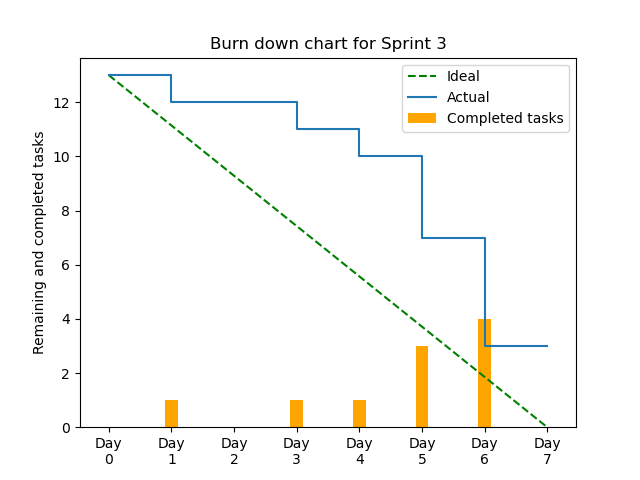
\includegraphics[scale=0.75]{Sprint03_BurnDownChart}  --- METTERE QUELLO CORRETTO!!! ---

        \end{itemize}

        \newpage
        \subsection{Sprint Retrospective (S06):}
        \begin{itemize}
            \item \textbf{Data:} 29/01/2023
            \newline \textbf{Durata:} 55 min.
            \newline \textbf{Partecipanti:} \treP \tre
            \newline
            \newline Si concorda che l'approccio Test Driven Design risulta efficiente soprattutto nel fare refactor del codice, quindi si decide di proseguire con questa metodologia, nonostante il costo iniziale. Inoltre si decide di continuare a fare Pair Programming e di introdurre in parte minore anche XP, poich\'e si \'e rivelato utile negli ultimi giorni di Sprint per fare il refactor di alcune porzioni di codice estese.
            \newline Si concorda che l'approccio di Pair Programming nella fase iniziale dello Sprint ha contribuito in modo significativo alla velocizzazione sia di produzione di codice per i nuovi developer, che di diffusione della conoscenza acquisita.
            \newline Viene ridiscusso l'ordine di dettaglio della Definition of Done. e viene concordato che la chiusura della Documentazione sarà spostata prima dell'accettazione della Pull Request. E' stato introdotto uno strumento per creare in automatico via script il Burndown Chart, recuperando le informazioni di stato direttamente da GitHub, via API.
        \end{itemize}

        \newpage
        %%%%%%%%%%%%%%%%%%
        %                %
        %    SPRINT 4    %
        %                %
        %%%%%%%%%%%%%%%%%%
        \section{SPRINT 04}
        \begin{itemize}
            \item Inizio sprint: \textit{30/01/2023}
            \item Fine sprint: \textit{5/02/2023}
        \end{itemize}
        \begin{itemize}
            \item \textbf{Sprint Goal (SG):} \\
            \begin{indent}
                \newline Il sistema deve permettere ad un utente di aggiungere le sue carte fisiche al proprio mazzo delle possedute e visualizzarle nella rispettiva sezione dei mazzi, oltre a proporre uno scambio di carte verso altri utenti del sistema e rimuovere le proprie carte fisiche dal mazzo delle possedute e dal mazzo delle desiderate.  \\
            \end{indent}
        \end{itemize}
        \begin{itemize}
            \item \textbf{Ruoli:}\\
            \textbf{Product Owner:} Alessia Crimaldi \\
            \textbf{Scrum Master:} Alessio Arcara \\
            textbf{Development team:} Matteo Sacco, Davide Fermi \\
        \end{itemize}
        \vspace{2mm} %5mm vertical space
        \subsection{Sprint Planning (S04)}
        \textbf{Data:} 29/01/2023\\
        \textbf{Durata:} 95 min.\\
        \textbf{Partecipanti:} \quattroP \quattro \\
        \newline La riunione non è stata caratterizzata da particolari cambiamenti rispetto al flusso collaudato dei precedenti Sprint Planning, basati su Planning Poker e con metodologia di stima basata sulla "velocity".

        \newpage
        \subsection{Stato board dopo lo Sprint Planning (S04):}
        \small
        \def\arraystretch{2}%
        \begin{tabular}{ | p{4.5cm} | p{5.5cm} | p{5.2cm} | p{5.8cm} | p{2cm}| }
            \hline
            \textbf{UC raffinati}
            & \textbf{Product Backlog}
            & \textbf{Sprint Backlog}
            & \textbf{Sprint In progress}
            & \textbf{Sprint Done} \\
            \hline
            \hline
            \textbf{UC01:} Come visitatore voglio selezionare un gioco e vedere l'elenco di tutte le sue carte
            &  \textbf{UC07:} Come utente voglio poter aggiungere le carte reali che desidero al mazzo delle desiderate  & \textbf{Task7 [UC06]\#105} Refactor di GsonSerializer e MapDB & \textbf{Task5 [UC05]\#57:} Modificare CardView per poter aggiungere la carta al mazzo delle possedute  & \\
            \hline
            \textbf{UC02:} Come visitatore voglio poter fare delle ricerche per vedere un elenco di carte filtrato
            &  \textbf{UC08:} Come utente voglio poter rimuovere le carte reali che non desidero più dal mazzo delle desiderate & \textbf{Task13 [UC09]\#117:} Popolare la lista 'Owned by' degli utenti in CardView & \textbf{Task2 [UC06]\#59:} Creare RPC per poter visualizzare la lista di carte reali contenute nel mazzo delle possedute  & \\
            \hline
            \textbf{UC03:} Come visitatore voglio selezionare una carta e vederne i dettagli
            & \textbf{UC10:} Come utente voglio poter accettare una richiesta di scambio di un altro utente & \textbf{Task12 [UC09]\#111:} Creare RPC per popolare la lista "Owned by" in Card Details view & \textbf{Task4 [UC06]\#61:} Creare pagina per visualizzare il mazzo delle possedute (Place, Activity e View) & \\
            \hline
            \textbf{UC04:}  Come utente voglio potermi autenticare per gestire i miei mazzi di carte & \textbf{UC12:} Come utente voglio poter rifiutare una richiesta di scambio di un altro utente & \textbf{Task1 [UC09]\#82:} Creare NewExchangePlace e pensare alla gestione dell'URI & & \\
            \hline
            \textbf{UC05:} Come utente voglio poter aggiungere le mie carte reali al mazzo delle possedute & \textbf{UC13:} Come utente voglio poter modificare le proprietà di una mia carta reale aggiunta al mazzo delle possedute & \textbf{Task2 [UC09]\#83:} Creare NewExchangeActivity, NewExchangeView inizialmente vuote & & \\
            \hline
            \textbf{UC06:} Come utente voglio poter visualizzare il contenuto del mazzo delle possedute & \textbf{UC14:} Come utente voglio poter proporre una richiesta di scambio per una o più carte reali desiderate da un altro utente  & \textbf{Task3 [UC09]\#85:} Creare collegamento tra CardPlace e NewExchangePlace (ha un'id della proposta che può essere null inizialmente) & & \\
            \hline
            \textbf{UC09:} Come utente voglio poter proporre una richiesta di scambio per una o più carte reali possedute da un altro utente &  & \textbf{Task4 [UC09]\#84:} Creare RPC per prendere le informazioni dei deck owned dell'utente mittente e utente destinatario & & \\
            \hline
            \textbf{UC11:} Come utente voglio poter rimuovere le mie carte reali dal mazzo delle possedute & & \textbf{Task5 [UC09]\#87:} Creare UI per definire la proposta di scambio tra utente mittente e utente destinatario & & \\
            \hline
            & & \textbf{Task6 [UC09]\#86:} Selezionare la carta fisica selezionata nella pagina precedente come già selezionata & & \\
            \hline
            & & --- continua --- & & \\
            \hline
        \end{tabular}

        \newpage
        \subsection{Stato board dopo lo Sprint Planning (S04):}
        \small
        \def\arraystretch{2}%
        \begin{tabular}{ | p{4.5cm} | p{5.5cm} | p{5.2cm} | p{5.8cm} | p{2cm}| }
            \hline
            \textbf{UC raffinati}
            & \textbf{Product Backlog}
            & \textbf{Sprint Backlog}
            & \textbf{Sprint In progress}
            & \textbf{Sprint Done} \\
            \hline
            \hline
            & & \textbf{Task7 [UC09]\#88:} Creare multi-selezione o nel caso sia già stata fatta, implementare la logica, per poi contattare il server con le liste delle carte selezionate & & \\
            \hline
            & & \textbf{Task8 [UC09]\#89:} Creare modello proposta (idProposta, emailMittente, emailDestinario, listaCarteMittente, listaCarteDestinatario) & & \\
            \hline
            & & \textbf{Task9 [UC09]\#90:} Creare mappa delle proposte su MapDB & & \\
            \hline
            & & \textbf{Task10 [UC09]\#91:} Creare RPC per salvare la proposta sulla mappa delle proposte & & \\
            \hline
            & & \textbf{Task11 [UC09]\#92:} Definire logica per contattare RPC con le informazioni della proposta di scambio & & \\
            \hline
            & & \textbf{Task1 [UC11]\#106:}  Creare RPC per rimuovere una carta fisica nel mazzo delle possedute dell'utente & & \\
            \hline
        \end{tabular}

        \newpage
        \normalsize
        \subsection{Daily Scrum (S04):}
        \begin{itemize}
            \item \textbf{Data:} 31/01/2023
            \newline \textbf{Durata:} 15 min.
            \newline \textbf{Partecipanti:} \quattro
            \newline \textbf{Percezione attuale dello SG:} Positiva (Dev 1)
        \end{itemize}
        \begin{itemize}
            \item \textbf{Data:} 01/02/2023
            \newline \textbf{Durata:} 15 min.
            \newline \textbf{Partecipanti:} \quattro
            \newline \textbf{Percezione attuale dello SG:} Negativa (Dev 1), Positiva (Dev 2)
        \end{itemize}
        \begin{itemize}
            \item \textbf{Data:} 02/02/2023
            \newline \textbf{Durata:} 15 min.
            \newline \textbf{Partecipanti:} \quattro
            \newline \textbf{Percezione attuale dello SG:} Negativa (Dev 1), Negativa (Dev 2)
        \end{itemize}
        \begin{itemize}
            \item \textbf{Data:} 03/02/2023
            \newline \textbf{Durata:} 15 min.
            \newline \textbf{Partecipanti:} \quattro
            \newline \textbf{Percezione attuale dello SG:} Negativa (Dev 1), Negativa (Dev 2)
        \end{itemize}
        \begin{itemize}
            \item \textbf{Data:} 04/02/2023
            \newline \textbf{Durata:} 12 min.
            \newline \textbf{Partecipanti:}  \quattro
            \newline \textbf{Percezione attuale dello SG:} Negativa (Dev 1), Negativa (Dev 2)
        \end{itemize}
        \begin{itemize}
            \item \textbf{Data:} 05/02/2023
            \newline \textbf{Durata:} 10 min.
            \newline \textbf{Partecipanti:}  \quattro
            \newline \textbf{Percezione attuale dello SG:} Negativa (Dev 1), Negativa (Dev 2)
        \end{itemize}
        \vspace{2mm} %5mm vertical space
        \textbf{Note:} Si è cercato di mantenere i daily entro i 10 minuti, nei quali il team di sviluppo, condotti dallo Scrum Master, espongono quanto fatto, quanto hanno in progetto di fare e i principali problemi riscontrati. Al termine, lo Scrum master chiede una percezione dello Sprint Goal e mostra il BurnDown Chart aggiornato.

        \newpage
        \subsection{Stato Board finale (S04):}
        \small
        \def\arraystretch{2}%
        \begin{tabular}{ | p{5cm} | p{5cm} | p{3cm} | p{3cm} | p{7cm}| }
            \hline
            \textbf{UC raffinati}
            & \textbf{Product Backlog}
            & \textbf{Sprint Backlog}
            & \textbf{Sprint In progress}
            & \textbf{Sprint Done} \\
            \hline
            \hline
            \textbf{UC01:} Come visitatore voglio selezionare un gioco e vedere l'elenco di tutte le sue carte
            &  \textbf{UC07:} Come utente voglio poter aggiungere le carte reali che desidero al mazzo delle desiderate  &  &  & \textbf{Task5 [UC05]\#57:} Modificare CardView per poter aggiungere la carta al mazzo delle possedute \\
            \hline
            \textbf{UC02:} Come visitatore voglio poter fare delle ricerche per vedere un elenco di carte filtrato
            &  \textbf{UC08:} Come utente voglio poter rimuovere le carte reali che non desidero più dal mazzo delle desiderate &  & &\textbf{Task2 [UC06]\#59:} Creare RPC per poter visualizzare la lista di carte reali contenute nel mazzo delle possedute \\
            \hline
            \textbf{UC03:} Come visitatore voglio selezionare una carta e vederne i dettagli
            & \textbf{UC10:} Come utente voglio poter accettare una richiesta di scambio di un altro utente &  & &\textbf{Task4 [UC06]\#61:} Creare pagina per visualizzare il mazzo delle possedute (Place, Activity e View) \\
            \hline
            \textbf{UC04:}  Come utente voglio potermi autenticare per gestire i miei mazzi di carte & \textbf{UC12:} Come utente voglio poter rifiutare una richiesta di scambio di un altro utente & & & \textbf{Task7 [UC06]\#105} Refactor di GsonSerializer e MapDB \\
            \hline
            \textbf{UC05:} Come utente voglio poter aggiungere le mie carte reali al mazzo delle possedute & \textbf{UC13:} Come utente voglio poter modificare le proprietà di una mia carta reale aggiunta al mazzo delle possedute & & & \textbf{Task1 [UC09]\#82:} Creare NewExchangePlace e pensare alla gestione dell'URI \\
            \hline
            \textbf{UC06:} Come utente voglio poter visualizzare il contenuto del mazzo delle possedute & \textbf{UC14:} Come utente voglio poter proporre una richiesta di scambio per una o più carte reali desiderate da un altro utente  & & &  \textbf{Task2 [UC09]\#83:} Creare NewExchangeActivity, NewExchangeView inizialmente vuote \\
            \hline
            \textbf{UC09:} Come utente voglio poter proporre una richiesta di scambio per una o più carte reali possedute da un altro utente &  \textbf{UC15:} Come utente voglio poter aggiungere le carte possedute ad un mazzo personalizzato   & & & \textbf{Task3 [UC09]\#85:} Creare collegamento tra CardPlace e NewExchangePlace (ha un'id della proposta che può essere null inizialmente)  \\
            \hline
            \textbf{UC11:} Come utente voglio poter rimuovere le mie carte reali dal mazzo delle possedute & \textbf{UC16:} Come utente voglio poter rimuovere le carte possedute da un mazzo personalizzato &  & &  \textbf{Task4 [UC09]\#84:} Creare RPC per prendere le informazioni dei deck owned dell'utente mittente e utente destinatario \\
            \hline
            & & --- continua --- & & \\
            \hline
        \end{tabular}

        \newpage
        \small
        \def\arraystretch{2}%
        \noindent
        \begin{tabular}{ | p{5cm} | p{5cm} | p{3cm} | p{3cm} | p{7cm}| }
            \hline
            \textbf{UC raffinati}
            & \textbf{Product Backlog}
            & \textbf{Sprint Backlog}
            & \textbf{Sprint In progress}
            & \textbf{Sprint Done} \\
            \hline
            \hline
            & \textbf{UC17:} Come utente voglio poter aggiungere un mazzo personalizzato  &  & & \textbf{Task5 [UC09]\#87:} Creare UI per definire la proposta di scambio tra utente mittente e utente destinatario \\
            \hline
            & \textbf{UC18:} Come utente voglio poter rimuovere un mazzo personalizzato  & & & \textbf{Task6 [UC09]\#86:} Selezionare la carta fisica selezionata nella pagina precedente come già selezionata\\
            \hline
            & \textbf{UC19:} Come utente voglio poter visualizzare le proposte di scambio & & & \textbf{Task7 [UC09]\#88:} Creare multi-selezione o nel caso sia già stata fatta, implementare la logica, per poi contattare il server con le liste delle carte selezionate  \\
            \hline
            & \textbf{UC20:} Come utente voglio poter modificare le proprietà di una mia carta reale aggiunta al mazzo delle desiderate & & & \textbf{Task8 [UC09]\#89:} Creare modello proposta (idProposta, emailMittente, emailDestinario, listaCarteMittente, listaCarteDestinatario)  \\
            \hline
            & \textbf{UC21:} Come utente voglio poter visualizzare i dettagli della proposta & & & \textbf{Task9 [UC09]\#90:} Creare mappa delle proposte su MapDB  \\
            \hline
            & & & & \textbf{Task10 [UC09]\#91:} Creare RPC per salvare la proposta sulla mappa delle proposte  \\
            \hline
            & & & & \textbf{Task11 [UC09]\#92:} Definire logica per contattare RPC con le informazioni della proposta di scambio  \\
            \hline
            & & & & \textbf{Task12 [UC09]\#111:} Creare RPC per popolare la lista "Owned by" in Card Details view  \\
            \hline
            & & & & \textbf{Task13 [UC09]\#117:} Popolare la lista 'Owned by' degli utenti in CardView  \\
            \hline
            & & & & \textbf{Task1 [UC11]\#106:}  Creare RPC per rimuovere una carta fisica nel mazzo delle possedute dell'utente \\
            \hline
        \end{tabular}


        \newpage
        \normalsize
        \subsection{Sprint Review (S04):}
        \begin{itemize}
            \item \textbf{Data:}5/02/2023
            \newline \textbf{Durata:} 95 min.
            \newline \textbf{Partecipanti:} \quattroP \quattro
            \newline
            \newline I developers mostrano al Product Owner una Demo di quanto prodotto. Si evidenzia come sia stato possibile completare tutte le attività e fornire un prodotto con nuove funzionalità. Il Product Owner decide che lo sprint si è concluso positivamente ed è possibile rilasciare, incaricando i developers delle pratiche formali di rilascio e della definizione delle Releas Notes.
            \newline Lo Scrum Master illustra il Burn Down chart e apre un confronto con il team riguardo allo sprint appena concluso.
            Si analizzano quindi le principali cause di rallentamento ed emergono in particolar modo alcuni aspetti sia legati alla pianificazione, come la presenza di task troppo grandi e difficilmente controllabili in termini di stima e gestione, sia aspetti legati all'implementazione, con la scoperta, durante la programmazione, di restrizioni e problematiche causate dalla poca documentazione disponibile per le librerie e framework utilizzati. Mentre questo secondo aspetto non è negoziabile, in quanto requisito obbligatorio, per il primo aspetto legato alla pianificazione si decide di migliorare il dettaglio della raffinazione delle user stories, in modo da avere molti task piccoli e più gestibili, anche in chiave di stima, rispetto a pochi task molto grandi.

            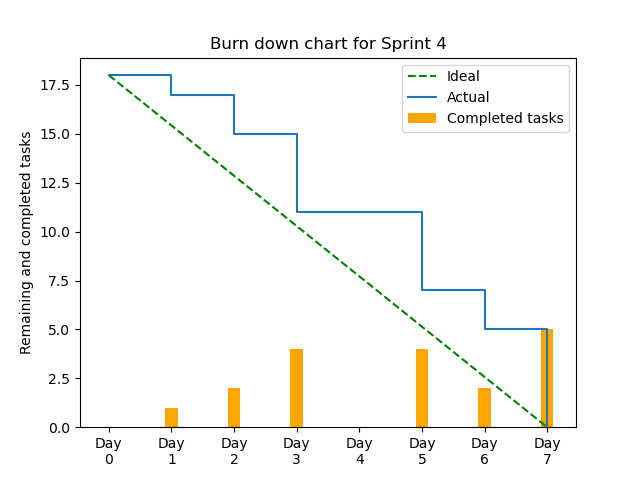
\includegraphics[scale=0.75]{Sprint04_BurnDownChart}

        \end{itemize}

        \newpage
        \subsection{Sprint Retrospective (S04):}
        \begin{itemize}
            \item \textbf{Data:} 5/02/2023
            \newline \textbf{Durata:} 60 min.
            \newline \textbf{Partecipanti:} \quattroP \quattro
            \newline
            \newline  Lo Scrum Master chiede a tutti i membri di evidenziare gli aspetti positivi dello sprint appena concluso. Si evidenzia come la flessibilità del metodo SCRUM abbia potuto portare delle tempestive azioni correttive in corsa, reagendo alla situazione creatasi ed evitando un blocco completo o il rischio di un fallimento dello Sprint, in quanto il carico di lavoro e lo stress avrebbero portato ad un ulteriore rallentamento della produttività.
            \newline Tale situazione ha portato comunque alcuni contrasti all'interno del team, in quanto essendo tutto prioritario (codice, documentazione e review), inevitabilmente qualcosa veniva in parte trascurato.
            Per evitare il ripetersi di queste situazioni in futuro, oltre a quanto già definito riguardo una maggior dettaglio di raffinazione delle user stories, Alessio introduce il concetto di "Pull Request Royal Rumble", ovvero che lo sviluppatore, come prima priorità, ha il dovere di verificare eventuali richieste di Code Review. Questo per evitare che il codice rimanga dimenticato in attesa per troppo tempo, aumentando quindi il rischio che richieda ennesime risoluzioni di conflitti con il branch principale e nuovo lavoro extra non preventivato, in questo caso evitabile, anticipando il prima possibile la Code Review.
        \end{itemize}

        \newpage
        %%%%%%%%%%%%%%%%%%
        %                %
        %    SPRINT 5    %
        %                %
        %%%%%%%%%%%%%%%%%%
        \section{SPRINT 05}
        \begin{itemize}
            \item Inizio sprint: \textit{06/02/2023}
            \item Fine sprint: \textit{12/02/2023}
        \end{itemize}
        \begin{itemize}
            \item \textbf{Sprint Goal (SG):}
            \begin{indent}
                \newline Il sistema deve permettere ad un utente di gestire le proprie carte fisiche nei propri mazzi delle carte possedute e desiderate. L'utente deve inoltre poter creare o eliminare uno o più mazzi personalizzati, inserendo o rimuovendo al loro interno carte fisiche possedute. Infine, il sistema deve poter permettere all'utente di visualizzare le proposte di scambio inviate e ricevute, e accettarle o rifiutarle.
            \end{indent}
        \end{itemize}
        \begin{itemize}
            \item \textbf{Ruoli:}\\
            \textbf{Product Owner:} Davide Fermi\\
            \textbf{Scrum Master:} Alessia Crimaldi\\
            \textbf{Development team:} Alessio Arcara, Matteo Sacco\\
        \end{itemize}
        \vspace{2mm} %5mm vertical space
        \subsection{Sprint Planning (S05)}
        \textbf{Data:} 05/01/2023\\
        \textbf{Durata:} 125 min.\\
        \textbf{Partecipanti:} \cinqueP \cinque\\
        \newline La riunione non è stata caratterizzata da particolari cambiamenti, rispetto al flusso collaudato dei precedenti Sprint Planning, basati su Poker Plain e con metodologia di stima basata sulla "velocity".

        \newpage
        \subsection{Stato board dopo lo Sprint Planning (S05):}
        \small
        \def\arraystretch{2}%
        \begin{tabular}{ | p{6.5cm} | p{3cm} | p{8cm} | p{2.9cm} | p{2.4cm}| }
            \hline
            \textbf{UC raffinati}
            & \textbf{Product Backlog}
            & \textbf{Sprint Backlog}
            & \textbf{Sprint In progress}
            & \textbf{Sprint Done} \\
            \hline
            \hline
            \textbf{UC01:}  Come visitatore voglio selezionare un gioco e vedere l'elenco di tutte le sue carte  & & \textbf{Task1[UC08]\#137} Collegare RPC removePhysicalCardFromDeck al click del tasto deleteButton del PhysicalCardWidget  & & \\ \hline
            \textbf{UC02:}  Come visitatore voglio poter fare delle ricerche per vedere un elenco di carte filtrato  & & \textbf{Task2[UC08]\#138} Nascondere deleteButton nella visualizzazione della proposta  & & \\ \hline
            \textbf{UC03:}  Come visitatore voglio selezionare una carta e vederne i dettagli  & & \textbf{Task1[UC10]\#98} Creare RPC per accettare la proposta di scambio, aggiornare i proprietari delle carte scambiate verificando che esistano ancora  & & \\ \hline
            \textbf{UC04:}   Come utente voglio potermi autenticare per gestire i miei mazzi di carte  & & \textbf{Task2[UC10]\#186} Creare metodo aggiuntivo per RPC di accettazione Proposta, per rimuovere da mazzo desiderate le carte fisiche con uno specifico cardId di catalogo e che hanno uno status minore o uguale alla carta scambiata  & & \\ \hline
            \textbf{UC05:}  Come utente voglio poter aggiungere le mie carte reali al mazzo delle possedute  & & \textbf{Task3[UC10]\#99} Contattare dal client l'RPC con l'id della proposta e con il token comunicando di aver accettato la proposta  & & \\ \hline
            \textbf{UC06:}  Come utente voglio poter visualizzare il contenuto del mazzo delle possedute  & & \textbf{Task4[UC10]\#100} E una volta accettata la proposta, far tornare alla pagina precedente  & & \\ \hline
            \textbf{UC09:}  Come utente voglio poter proporre una richiesta di scambio per una o più carte reali possedute da un altro utente  & & \textbf{Task2[UC11]\#137} Collegare RPC removePhysicalCardFromDeck al click del tasto deleteButton del PhysicalCardWidget  & & \\ \hline
            \textbf{UC11:}  Come utente voglio poter rimuovere le mie carte reali dal mazzo delle possedute  & & \textbf{Task3[UC11]\#138} Nascondere deleteButton nella visualizzazione della proposta  & & \\ \hline
            \textbf{UC07:}  Come utente voglio poter aggiungere le carte reali che desidero al mazzo delle desiderate   & & \textbf{Task4[UC11]\#128} Verificare se la carta reale eliminata è presente in uno o più mazzi personalizzati e rimuoverla  & & \\ \hline
            & & --- continua --- & & \\
            \hline
        \end{tabular}
        \newpage
        \small
        \noindent
        \def\arraystretch{2}%
        \begin{tabular}{ | p{6.5cm} | p{3cm} | p{8cm} | p{2.9cm} | p{2.4cm}| }
            \hline
            \textbf{UC raffinati}
            & \textbf{Product Backlog}
            & \textbf{Sprint Backlog}
            & \textbf{Sprint In progress}
            & \textbf{Sprint Done} \\
            \hline
            \hline
            \textbf{UC08:}  Come utente voglio poter rimuovere le carte reali che non desidero più dal mazzo delle desiderate  & & \textbf{Task1[UC12]\#144} Creare RPC per rifiutare una proposta ricevuta  & & \\ \hline
            \textbf{UC10:}  Come utente voglio poter accettare una richiesta di scambio di un altro utente  & & \textbf{Task2[UC12]\#145} Contattare RPC con id e token da refuseButton per rifiutare la proposta ricevuta  & & \\ \hline
            \textbf{UC12:}  Come utente voglio poter rifiutare una richiesta di scambio di un altro utente  & & \textbf{Task3[UC12]\#146} Capire se è possibile portare l'utente alla pagina precedente  & & \\ \hline
            \textbf{UC13:}  Come utente voglio poter modificare le proprietà di una mia carta reale aggiunta al mazzo delle possedute  & & \textbf{Task4[UC12]\#147} Una volta rifiutata la proposta mostrare un alert di avvenuto rifiuto e all'okay portarlo alla pagina precedente  & & \\ \hline
            \textbf{UC14:}  Come utente voglio poter proporre una richiesta di scambio per una o più carte reali desiderate da un altro utente   & & \textbf{Task1[UC13]\#157} Creare RPC passando token, id della carta fisica, nuovo status e nuova descrizione per modificare le proprietà della carta  & & \\ \hline
            \textbf{UC15:}  Come utente voglio poter aggiungere le carte possedute ad un mazzo personalizzato    & & \textbf{Task2[UC13]\#171} Modificare RPC inserendo la logica per modificare la carta fisica non solo nel mazzo delle possedute ma anche in tutti i mazzi personalizzati in cui essa è contenuta, restituendo la lista dei mazzi modificati  & & \\ \hline
            \textbf{UC16:}  Come utente voglio poter rimuovere le carte possedute da un mazzo personalizzato  & & \textbf{Task3[UC13]\#158} Rendere editabile PhysicalCardWidget per modificare le proprietà della carta nel mazzo delle carte possedute  & & \\ \hline
            \textbf{UC17:}  Come utente voglio poter aggiungere un mazzo personalizzato   & & \textbf{Task4[UC13]\#159} Rendere editabile PhysicalCardWidget solo nel mazzo delle carte possedute e delle desiderate non negli altri mazzi  & & \\ \hline
            \textbf{UC18:}  Come utente voglio poter rimuovere un mazzo personalizzato   & & \textbf{Task5[UC13]\#161} Contattare RPC lato client per modificare stato e descrizione della carta fisica e aggiornare i campi stato e descrizione della carta fisica nel mazzo delle possedute o delle desiderate  & & \\ \hline
            & & --- continua --- & & \\
            \hline
        \end{tabular}
        \newpage
        \small
        \noindent
        \def\arraystretch{2}%
        \begin{tabular}{ | p{6.5cm} | p{3cm} | p{8cm} | p{2.9cm} | p{2.4cm}| }
            \hline
            \textbf{UC raffinati}
            & \textbf{Product Backlog}
            & \textbf{Sprint Backlog}
            & \textbf{Sprint In progress}
            & \textbf{Sprint Done} \\
            \hline
            \hline
            \textbf{UC19:}  Come utente voglio poter visualizzare le proposte di scambio & & \textbf{Task6[UC13]\#173} Se la carta modificata è inserita in mazzi personalizzati, aggiornare le informazioni della carta anche nei mazzi personalizzati  & & \\ \hline
            \textbf{UC20:}  Come utente voglio poter modificare le proprietà di una mia carta reale aggiunta al mazzo delle desiderate & & \textbf{Task1[UC14]\#140} Popolare lista degli utenti che desiderano la carta  & & \\ \hline
            \textbf{UC21:}  Come utente voglio poter visualizzare i dettagli della proposta & & \textbf{Task2[UC14]\#118} Creare RPC per restituzione id cartafisica Posseduta per ogni cartafisica desiderata in dettaglio card, con parametri cardId di catalogo, game e token, per abilitare tasto exchange in Wished By list in card detail e passare controproposta  & & \\ \hline
            & & \textbf{Task3[UC14]\#141} Disabilitare i pulsanti exchange nella lista degli utenti che la desiderano se l'utente non ha quella carta  & & \\ \hline
            & & \textbf{Task4[UC14]\#142} Preselezionare la carta del mazzo delle possedute del mittente che il destinatario desidera  & & \\ \hline
            & & \textbf{Task2[UC15]\#153} Creare nuova RPC per inserimento multiplo di carte fisiche in mazzo personalizzato restituendo lista carte fisiche di quel mazzo  & & \\ \hline
            & & \textbf{Task3[UC15]\#154} Creare bottone nel mazzo personalizzato e gestire multi-selezione per aggiunta carta/e fisiche selezionate dal mazzo possedute  & & \\ \hline
            & & \textbf{Task4[UC15]\#155} Contattare RPC inviando token, lista carta/e fisica/e, nome mazzo personalizzato  & & \\ \hline
            & & \textbf{Task5[UC15]\#156} Aggiornare la pagina dei mazzi con le carte fisiche aggiunte ai mazzi personalizzati  & & \\ \hline
            & & \textbf{Task2[UC17]\#148} Contattare RPC addDeck da deckView per aggiungere il mazzo personalizzato con token e nome del mazzo scelto  & & \\ \hline
            & & --- continua --- & & \\
            \hline
        \end{tabular}
        \newpage
        \small
        \noindent
        \def\arraystretch{2}%
        \begin{tabular}{ | p{6.5cm} | p{3cm} | p{8cm} | p{2.9cm} | p{2.4cm}| }
            \hline
            \textbf{UC raffinati}
            & \textbf{Product Backlog}
            & \textbf{Sprint Backlog}
            & \textbf{Sprint In progress}
            & \textbf{Sprint Done} \\
            \hline
            \hline
            & & \textbf{Task3[UC17]\#149} Aggiungere il mazzo creato alla pagina dei mazzi  & & \\ \hline
            & & \textbf{Task1[UC18]\#150} Creare RPC passando token e nome del mazzo per rimuovere un mazzo personalizzato  & & \\ \hline
            & & \textbf{Task2[UC18]\#151} Aggiungere pulsante a DeckWidget (non visibile se è il mazzo delle carte reali possedute e delle desiderate) per rimuovere il mazzo personalizzato  & & \\ \hline
            & & \textbf{Task3[UC18]\#152} Contattare RPC removeCustomDeck e rimuovere il mazzo dalla pagina dei deck  & & \\ \hline
            & & \textbf{Task1[UC19]\#94} Creare RPC per vedere la lista delle proposte di scambio ricevute  & & \\ \hline
            & & \textbf{Task2[UC19]\#131} Creare RPC per vedere la lista delle proposte di scambio effettuate  & & \\ \hline
            & & \textbf{Task3[UC19]\#132} Creare hyperlink nella sidebar, exchangesLink in route constants, ExchangesPlace e modificare AppPlaceHistoryMapper  & & \\ \hline
            & & \textbf{Task4[UC19]\#133} Creare ExchangesActivity, ExchangesView inizialmente vuote  & & \\ \hline
            & & \textbf{Task5[UC19]\#134} Creare ProposalListWidget della lista delle proposte e impostare UI pagina delle proposte  & & \\ \hline
            & & \textbf{Task6[UC19]\#135} Contattare RPC per popolare lista proposte effettuate  & & \\ \hline
            & & \textbf{Task7[UC19]\#187} Contattare RPC per popolare lista proposte ricevute  & & \\ \hline
            & & \textbf{Task8[UC19]\#136} Una volta cliccato una proposta, l'utente dovrà essere portato nella pagina della proposta  & & \\ \hline
            & & --- continua --- & & \\
            \hline
        \end{tabular}
        \newpage
        \small
        \noindent
        \def\arraystretch{2}%
        \begin{tabular}{ | p{6.5cm} | p{3cm} | p{8cm} | p{2.9cm} | p{2.4cm}| }
            \hline
            \textbf{UC raffinati}
            & \textbf{Product Backlog}
            & \textbf{Sprint Backlog}
            & \textbf{Sprint In progress}
            & \textbf{Sprint Done} \\
            \hline
            \hline
            & & \textbf{Task1[UC21]\#93} Creare ExchangesPlace e pensare all'URI per vedere la proposta di scambio & & \\ \hline
            & & \textbf{Task2[UC21]\#95} Creare RPC per popolare la pagina della proposta di scambio  & & \\ \hline
            & & \textbf{Task3[UC21]\#96} Creare ExchangeActivity e scegliere se utilizzare NewExchangeView o creare una nuova view per visualizzare proposta di scambio  & & \\ \hline
            & & \textbf{Task4[UC21]\#97} Popolare ExchangeActivity e la view ad essa associata con i dati ottenuti dalla RPC getExchangeById  & & \\ \hline
            & & \textbf{Task5[UC21]\#179} Non rendere cliccabili le carte relative alla proposta di scambio  & & \\ \hline


            \hline
        \end{tabular}

        \newpage
        \normalsize
        \subsection{Daily Scrum (S05):}
        \begin{itemize}
            \item \textbf{Data:} 06/01/2023
            \newline \textbf{Durata:} 10 min.
            \newline \textbf{Partecipanti:} \cinque
            \newline \textbf{Percezione attuale dello SG:} Positiva (Dev 1), Negativa (Dev2)
        \end{itemize}
        \begin{itemize}
            \item \textbf{Data:} 07/01/2023
            \newline \textbf{Durata:} 15 min.
            \newline \textbf{Partecipanti:} \cinque
            \newline \textbf{Percezione attuale dello SG:} Positiva (Dev 1), Negativa (Dev 2)
        \end{itemize}
        \begin{itemize}
            \item \textbf{Data:} 08/01/2023
            \newline \textbf{Durata:} 10 min.
            \newline \textbf{Partecipanti:} \cinque
            \newline \textbf{Percezione attuale dello SG:} Positiva (Dev 1), Negativa (Dev 2)
        \end{itemize}
        \begin{itemize}
            \item \textbf{Data:} 09/01/2023
            \newline \textbf{Durata:} 10 min.
            \newline \textbf{Partecipanti:} \cinque
            \newline \textbf{Percezione attuale dello SG:} Positiva (Dev 1), Negativa (Dev 2)
        \end{itemize}
        \begin{itemize}
            \item \textbf{Data:} 10/01/2023
            \newline \textbf{Durata:} 12 min.
            \newline \textbf{Partecipanti:} \cinque
            \newline \textbf{Percezione attuale dello SG:} Positiva (Dev 1), Negativa (Dev 2)
        \end{itemize}
        \begin{itemize}
            \item \textbf{Data:} 11/01/2023
            \newline \textbf{Durata:} 10 min.
            \newline \textbf{Partecipanti:} \cinque
            \newline \textbf{Percezione attuale dello SG:} Positiva (Dev 1), Negativa (Dev 2)
        \end{itemize}

        \newpage
        \subsection{Stato Board finale (S05):}
        \small
        \def\arraystretch{2}%
        \begin{tabular}{ | p{7cm} | p{3cm} | p{2.8cm} | p{3cm} | p{7.2cm}| }
            \hline
            \textbf{UC raffinati}
            & \textbf{Product Backlog}
            & \textbf{Sprint Backlog}
            & \textbf{Sprint In progress}
            & \textbf{Sprint Done} \\
            \hline
            \hline
            \textbf{UC01:}  Come visitatore voglio selezionare un gioco e vedere l'elenco di tutte le sue carte  & &  & & \textbf{Task1[UC08]\#137} Collegare RPC removePhysicalCardFromDeck al click del tasto deleteButton del PhysicalCardWidget   \\ \hline
            \textbf{UC02:}  Come visitatore voglio poter fare delle ricerche per vedere un elenco di carte filtrato  & &  & & \textbf{Task2[UC08]\#138} Nascondere deleteButton nella visualizzazione della proposta   \\ \hline
            \textbf{UC03:}  Come visitatore voglio selezionare una carta e vederne i dettagli  & &  & & \textbf{Task1[UC10]\#98} Creare RPC per accettare la proposta di scambio, aggiornare i proprietari delle carte scambiate verificando che esistano ancora   \\ \hline
            \textbf{UC04:}   Come utente voglio potermi autenticare per gestire i miei mazzi di carte  & &  & & \textbf{Task2[UC10]\#186} Creare metodo aggiuntivo per RPC di accettazione Proposta, per rimuovere da mazzo desiderate le carte fisiche con uno specifico cardId di catalogo e che hanno uno status minore o uguale alla carta scambiata   \\ \hline
            \textbf{UC05:}  Come utente voglio poter aggiungere le mie carte reali al mazzo delle possedute  & &  & & \textbf{Task3[UC10]\#99} Contattare dal client l'RPC con l'id della proposta e con il token comunicando di aver accettato la proposta   \\ \hline
            \textbf{UC06:}  Come utente voglio poter visualizzare il contenuto del mazzo delle possedute  & &  & & \textbf{Task4[UC10]\#100} E una volta accettata la proposta, far tornare alla pagina precedente   \\ \hline
            \textbf{UC09:}  Come utente voglio poter proporre una richiesta di scambio per una o più carte reali possedute da un altro utente  & &  & & \textbf{Task2[UC11]\#137} Collegare RPC removePhysicalCardFromDeck al click del tasto deleteButton del PhysicalCardWidget   \\ \hline
            \textbf{UC11:}  Come utente voglio poter rimuovere le mie carte reali dal mazzo delle possedute  & &  & & \textbf{Task3[UC11]\#138} Nascondere deleteButton nella visualizzazione della proposta   \\ \hline
            \textbf{UC07:}  Come utente voglio poter aggiungere le carte reali che desidero al mazzo delle desiderate   & &  & & \textbf{Task4[UC11]\#128} Verificare se la carta reale eliminata è presente in uno o più mazzi personalizzati e rimuoverla   \\ \hline
            & & --- continua --- & & \\
            \hline
        \end{tabular}
        \newpage
        \small
        \noindent
        \def\arraystretch{2}%
        \begin{tabular}{ | p{7cm} | p{3cm} | p{2.8cm} | p{3cm} | p{7.2cm}| }
            \hline
            \textbf{UC raffinati}
            & \textbf{Product Backlog}
            & \textbf{Sprint Backlog}
            & \textbf{Sprint In progress}
            & \textbf{Sprint Done} \\
            \hline
            \hline
            \textbf{UC08:}  Come utente voglio poter rimuovere le carte reali che non desidero più dal mazzo delle desiderate  & &  & & \textbf{Task1[UC12]\#144} Creare RPC per rifiutare una proposta ricevuta   \\ \hline
            \textbf{UC10:}  Come utente voglio poter accettare una richiesta di scambio di un altro utente  & &  & & \textbf{Task2[UC12]\#145} Contattare RPC con id e token da refuseButton per rifiutare la proposta ricevuta   \\ \hline
            \textbf{UC12:}  Come utente voglio poter rifiutare una richiesta di scambio di un altro utente  & &  & & \textbf{Task3[UC12]\#146} Capire se è possibile portare l'utente alla pagina precedente   \\ \hline
            \textbf{UC13:}  Come utente voglio poter modificare le proprietà di una mia carta reale aggiunta al mazzo delle possedute  & &  & & \textbf{Task4[UC12]\#147} Una volta rifiutata la proposta mostrare un alert di avvenuto rifiuto e all'okay portarlo alla pagina precedente   \\ \hline
            \textbf{UC14:}  Come utente voglio poter proporre una richiesta di scambio per una o più carte reali desiderate da un altro utente   & &  & & \textbf{Task1[UC13]\#157} Creare RPC passando token, id della carta fisica, nuovo status e nuova descrizione per modificare le proprietà della carta   \\ \hline
            \textbf{UC15:}  Come utente voglio poter aggiungere le carte possedute ad un mazzo personalizzato    & &  & & \textbf{Task2[UC13]\#171} Modificare RPC inserendo la logica per modificare la carta fisica non solo nel mazzo delle possedute ma anche in tutti i mazzi personalizzati in cui essa è contenuta, restituendo la lista dei mazzi modificati   \\ \hline
            \textbf{UC16:}  Come utente voglio poter rimuovere le carte possedute da un mazzo personalizzato  & &  & & \textbf{Task3[UC13]\#158} Rendere editabile PhysicalCardWidget per modificare le proprietà della carta nel mazzo delle carte possedute   \\ \hline
            \textbf{UC17:}  Come utente voglio poter aggiungere un mazzo personalizzato   & &  & & \textbf{Task4[UC13]\#159} Rendere editabile PhysicalCardWidget solo nel mazzo delle carte possedute e delle desiderate non negli altri mazzi   \\ \hline
            \textbf{UC18:}  Come utente voglio poter rimuovere un mazzo personalizzato   & &  & & \textbf{Task5[UC13]\#161} Contattare RPC lato client per modificare stato e descrizione della carta fisica e aggiornare i campi stato e descrizione della carta fisica nel mazzo delle possedute o delle desiderate   \\ \hline
            & & --- continua --- & & \\
            \hline
        \end{tabular}
        \newpage
        \small
        \noindent
        \def\arraystretch{2}%
        \begin{tabular}{ | p{7cm} | p{3cm} | p{2.8cm} | p{3cm} | p{7.2cm}| }
            \hline
            \textbf{UC raffinati}
            & \textbf{Product Backlog}
            & \textbf{Sprint Backlog}
            & \textbf{Sprint In progress}
            & \textbf{Sprint Done} \\
            \hline
            \hline
            \textbf{UC19:}  Come utente voglio poter visualizzare le proposte di scambio & &  & & \textbf{Task6[UC13]\#173} Se la carta modificata è inserita in mazzi personalizzati, aggiornare le informazioni della carta anche nei mazzi personalizzati   \\ \hline
            \textbf{UC20:}  Come utente voglio poter modificare le proprietà di una mia carta reale aggiunta al mazzo delle desiderate & &  & & \textbf{Task1[UC14]\#140} Popolare lista degli utenti che desiderano la carta   \\ \hline
            \textbf{UC21:}  Come utente voglio poter visualizzare i dettagli della proposta & &  & & \textbf{Task2[UC14]\#118} Creare RPC per restituzione id cartafisica Posseduta per ogni cartafisica desiderata in dettaglio card, con parametri cardId di catalogo, game e token, per abilitare tasto exchange in Wished By list in card detail e passare controproposta   \\ \hline
            & &  & & \textbf{Task3[UC14]\#141} Disabilitare i pulsanti exchange nella lista degli utenti che la desiderano se l'utente non ha quella carta   \\ \hline
            & &  & & \textbf{Task4[UC14]\#142} Preselezionare la carta del mazzo delle possedute del mittente che il destinatario desidera   \\ \hline
            & &  & & \textbf{Task2[UC15]\#153} Creare nuova RPC per inserimento multiplo di carte fisiche in mazzo personalizzato restituendo lista carte fisiche di quel mazzo   \\ \hline
            & &  & & \textbf{Task3[UC15]\#154} Creare bottone nel mazzo personalizzato e gestire multi-selezione per aggiunta carta/e fisiche selezionate dal mazzo possedute   \\ \hline
            & &  & & \textbf{Task4[UC15]\#155} Contattare RPC inviando token, lista carta/e fisica/e, nome mazzo personalizzato   \\ \hline
            & & --- continua --- & & \\
            \hline
        \end{tabular}
        \newpage
        \small
        \noindent
        \def\arraystretch{2}%
        \begin{tabular}{ | p{7cm} | p{3cm} | p{2.8cm} | p{3cm} | p{7.2cm}| }
            \hline
            \textbf{UC raffinati}
            & \textbf{Product Backlog}
            & \textbf{Sprint Backlog}
            & \textbf{Sprint In progress}
            & \textbf{Sprint Done} \\
            \hline
            \hline
            & &  & & \textbf{Task5[UC15]\#156} Aggiornare la pagina dei mazzi con le carte fisiche aggiunte ai mazzi personalizzati   \\ \hline
            & &  & & \textbf{Task2[UC17]\#148} Contattare RPC addDeck da deckView per aggiungere il mazzo personalizzato con token e nome del mazzo scelto   \\ \hline
            & &  & & \textbf{Task3[UC17]\#149} Aggiungere il mazzo creato alla pagina dei mazzi   \\ \hline
            & &  & & \textbf{Task1[UC18]\#150} Creare RPC passando token e nome del mazzo per rimuovere un mazzo personalizzato   \\ \hline
            & &  & & \textbf{Task2[UC18]\#151} Aggiungere pulsante a DeckWidget (non visibile se è il mazzo delle carte reali possedute e delle desiderate) per rimuovere il mazzo personalizzato   \\ \hline
            & &  & & \textbf{Task3[UC18]\#152} Contattare RPC removeCustomDeck e rimuovere il mazzo dalla pagina dei deck   \\ \hline
            & &  & & \textbf{Task1[UC19]\#94} Creare RPC per vedere la lista delle proposte di scambio ricevute   \\ \hline
            & &  & & \textbf{Task2[UC19]\#131} Creare RPC per vedere la lista delle proposte di scambio effettuate   \\ \hline
            & &  & & \textbf{Task3[UC19]\#132} Creare hyperlink nella sidebar, exchangesLink in route constants, ExchangesPlace e modificare AppPlaceHistoryMapper   \\ \hline
            & &  & & \textbf{Task4[UC19]\#133} Creare ExchangesActivity, ExchangesView inizialmente vuote   \\ \hline
            & & --- continua --- & & \\
            \hline
        \end{tabular}
        \newpage
        \small
        \noindent
        \def\arraystretch{2}%
        \begin{tabular}{ | p{7cm} | p{3cm} | p{2.8cm} | p{3cm} | p{7.2cm}| }
            \hline
            \textbf{UC raffinati}
            & \textbf{Product Backlog}
            & \textbf{Sprint Backlog}
            & \textbf{Sprint In progress}
            & \textbf{Sprint Done} \\
            \hline
            \hline
            & &  & & \textbf{Task5[UC19]\#134} Creare ProposalListWidget della lista delle proposte e impostare UI pagina delle proposte   \\ \hline
            & &  & & \textbf{Task6[UC19]\#135} Contattare RPC per popolare lista proposte effettuate   \\ \hline
            & &  & & \textbf{Task7[UC19]\#187} Contattare RPC per popolare lista proposte ricevute   \\ \hline
            & &  & & \textbf{Task8[UC19]\#136} Una volta cliccato una proposta, l'utente dovrà essere portato nella pagina della proposta   \\ \hline
            & &  & & \textbf{Task1[UC21]\#93} Creare ExchangesPlace e pensare all'URI per vedere la proposta di scambio   \\ \hline
            & &  & & \textbf{Task2[UC21]\#95} Creare RPC per popolare la pagina della proposta di scambio   \\ \hline
            & &  & & \textbf{Task3[UC21]\#96} Creare ExchangeActivity e scegliere se utilizzare NewExchangeView o creare una nuova view per visualizzare proposta di scambio   \\ \hline
            & &  & & \textbf{Task4[UC21]\#97} Popolare ExchangeActivity e la view ad essa associata con i dati ottenuti dalla RPC getExchangeById   \\ \hline
            & &  & & \textbf{Task5[UC21]\#179} Non rendere cliccabili le carte relative alla proposta di scambio   \\ \hline

        \end{tabular}

        \newpage
        \normalsize
        \subsection{Sprint Review (S05):}
        \begin{itemize}
            \item \textbf{Data:} 12/02/2023
            \newline \textbf{Durata:} 105 min.
            \newline \textbf{Partecipanti:} \unoP \uno
            \newline
            \newline (TO-DO) I developers mostrano al PO una demo di quanto prodotto. Si evidenzia come non sia stato possibile sviluppare tutte le funzioni richieste dallo Sprint Goal. Si analizzano quindi le principali cause che hanno portato a questo problema, evidenziando come il framework GWT abbia portato della complessità nell'impementazione. Il PO decide quindi che non ci sono le condizioni sufficienti per procedere ad un rilascio, comprendendo le difficoltà riscontrate, ma chiedendo uno sforzo maggiore nello sprint successivo per poter raggiungere un prodotto rilasciabile. Non vengono evidenziati particolari problematiche di collaborazione e comunicazione all'interno del team.

            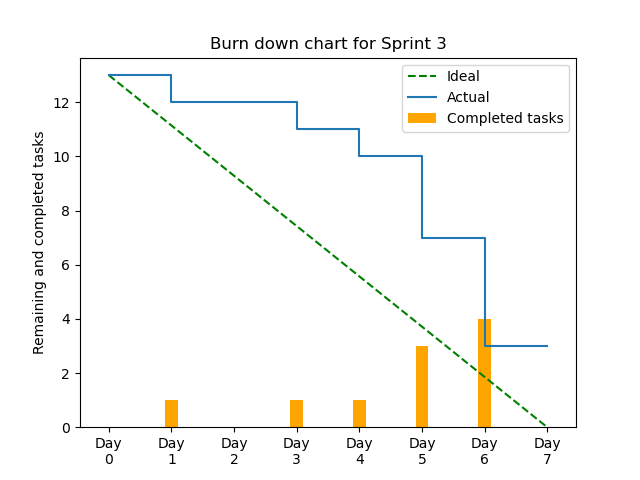
\includegraphics[scale=0.8]{Sprint03_BurnDownChart}
            --- METTERE QUELLO CORRETTO!!! ---
        \end{itemize}

        \newpage
        \subsection{Sprint Retrospective (S05):}
        \begin{itemize}
            \item \textbf{Data:} 12/02/2023
            \newline \textbf{Durata:} 70 min.
            \newline \textbf{Partecipanti:} \unoP \uno
            \newline
            \newline (TO-DO) Lo Scrum Master chiede a tutti i membri di evidenziare gli aspetti positivi dello sprint appena concluso. Si riconosce come il lavoro di formazione durante la fase di inception abbia reso più veloce lo sviluppo, ma non abbastanza. Per quanto riguarda gli aspetti negativi, emerge, oltre a quanto già discusso nella review, che nonostante la percezione sia quasi da subito parsa negativa, non è stata applicata nessuna azione correttiva. Si decide quindi per il futuro, qualora si ripresentasse una situazione simile, di richiedere un confronto con il Product Owner e valutare se sia necessario rivedere lo Sprint Backlog, nel tentativo di migliorare dinamicamente il flusso di lavoro.
        \end{itemize}
    \end{landscape}
\end{document}